\documentclass[a4paper,12pt]{report}
\usepackage{unifrsr}
\usepackage{hsc_texstyle}
\usepackage{hyperref}
\usepackage[style=alphabetic, backend=bibtex]{biblatex}
\addbibresource{references.bib}

\begin{document}
	\seminartitle{Human Smart Cities Seminar} % The title of the seminar

	\title{Wisdom of the Crowds \\ Can Crowd-Sourcing coexist with today’s Data Security Regulations?} % The title of your project

	\author{Pascal Gerig (16-104-721)\thanks{\email{pascal.gerig@students.unibe.ch}, University of Bern}
   		\and Lorenzo Wipfli  (13-933-262)\thanks{\email{lorenzo.wipfli@students.unibe.ch}, University of Bern}
   		\and Marcel Zauder  (16-124-836)\thanks{\email{marcel.zauder@students.unibe.ch}, University of Bern}
   	}	% Note: XX-XXX-XXX is the student's matriculation number
   	% The author(s), separated by \and

	\supervisor{Prof. Edy Portmann} % Name of the supervisor

	\assistant{Moreno Colombo \and Jhonny Pincay} %Name of the assistant(s)

	\date{\today} % Note: if this is left out, today's date will be used, this is the submission date!

	\maketitle

	\begin{abstract}
		This package, \textsf{unifrsr}, allows the easy creation of seminar
		reports using standard \LaTeX. It should be the last
		package loaded, to ensure that nothing overrides the page layout.

		Note that utility commands are available: 
		\begin{itemize}
			\item \verb+\seminartitle+ which specifies, optionally, the title of the seminar the report is being written for
			\item \verb+\supervisor+ which specifies the name of the professor supervisor of the project
			\item \verb+\assistant+ which specifies, optionally, the name of the assistants of the seminar, separated by the command \verb+\and+
		\end{itemize}

		\keywords{Seminar report, Human-IST Research Institute}
	\end{abstract}

	\tableofcontents

	\chapter{Example Chapter}
		This is an example of a section. As you see, it is just a standard {\LaTeX} section. Here is a footnote%
		\footnote{This is a footnote}.

		\section{Background and Motivation}
		\startsection
			It's all standard \LaTeX, as you can see. This is a very nice paper:
			\nocite{*}
		\closesection

	\chapter{Introduction}
		\section{Background and Motivation}
		\startsection
			Wisdom of the Crowd is the idea, that large collectives are supperior to individual experts in problem-solving, decision-making, innovating, and predicting \footnote{\url{https://www.investopedia.com/terms/w/wisdom-crowds.asp}}. 
			Human Smart Cities have an enormous interest in extracting the Wisdom of the Crowd as a foundation for better decision making.
			One suitable and broadly applied approach is crowd sourcing.
			Since data protection regulations are in effect across the world, crowd sourcing comes at a risk: if one does not comply with the relevant regulations, sanctions might be applied.
			This conflict is particularly topical, since the General Data Protection Regulation, referred to as GDPR, came into effect across the European Union in 2018.
			As Figure \ref{fig:enforcement_tracker} shows, enforcement activities have started to roll in over the past year. This forces in particular European (but potentially also other) Cities to comply with the GDPR.
		\closesection

		\section{Problem Statement and Research Question}
		\startsection
			\begin{enumerate}
				\item What methods do exist in order to gather information from citizen?
				\item What aspects do Human Smart Cities need to consider in order to comply with GDPR?
			\end{enumerate}
		\closesection
	
	\chapter{Methodology}
	
	\section{Nokia AVA}
	\startsection
	\subsection{Case studies}
	\closesection	
	\section{Others}
	\startsection
	\closesection
	\chapter{General Data Protection Regulation}
	\chaptermark{GDPR}
	The General Data Protection Regulation, referred to as GDPR, is in effect across the European Union from May 25, 2018.
	The Regulation is directly applicable to processing of personal data in the European Union and data collected from its data subjects.
	One central aspect of the regulation is, that it inludes a significant escalation in potential penalties (up to 4\% of the global revenue).
	Figure \ref{fig:enforcement_tracker} shows how enforcement activities increase from commencement until October 2021.
	For instance, Amazon was fined 746 million \texteuro \ in July 2021 \cite{EnforcementTracker}
	\begin{figure}
		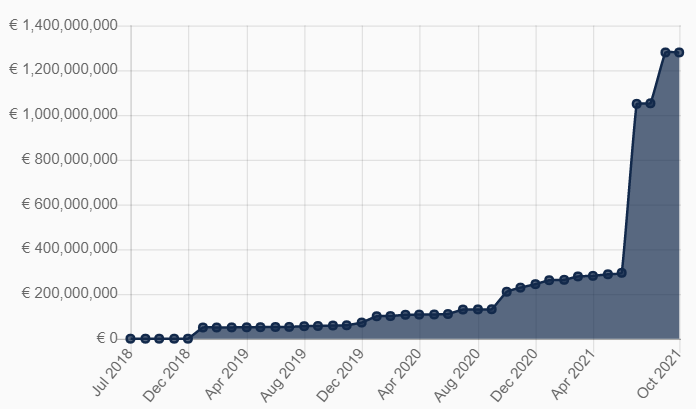
\includegraphics{EnforcementTracker_21-10-12.PNG}
		\caption{Enforcement activities \cite{EnforcementTracker}}
		\label{fig:enforcement_tracker}
	\end{figure}
	
	\section{Core Concepts}
	\startsection
	GDPR defines certain core concepts which are important for the further understanding of the regulation.\\
	\textbf{Personal data} is any information relating to an identified or identifieable natural person.
	There are three subtypes of interest to personal data. 
	First of, \textbf{sensible data} is defined as personal data that is revealing race, ethnic origin, political opinions, religious or philosophical beliefs, trade union membership, health, sex life and sexual orientation, genetic data or biometric data.
	Next, there is data relating to \textbf{criminal offences} and convictions.
	Finally, \textbf{health data} is personal data relating to physical or mental health of an individual, including the provision of healt care services, which reveal information about his or her health status.\\
	\textbf{Pseudonymization} is the processing of personal data in such a manner that the personal data can no longer be attributed to a specific data subject without the use of additional information, provided that such additional information is kept separately and is subject to technical and organisational measures to ensure that the personal data are not attributed to an identified or identifieable natural person.
	\textbf{Anonymization} eliminates personal data so that data subjects can no longer be identified. 
	Anonymized data is excluded from GDPR altogether because anonymized data is no longer personal data.
	\textbf{Data processing} means any operation or set of operations performed upon personal data or sets of personal data, whether or not by automated means, such as collection, recording, organisation, structuring, storage, adaptation or alternation, retrieval, consultation, use, disclosure by transmission, dissemination or otherwise making available, alignment or combination, restriction, erasure or destruction.
	\closesection

	\section{Data Processing Entities}
	\startsection
	The GDPR defines different entities responsible for data processing. These entities have different responsibilites.
	Namely there are the following:
	\begin{enumerate}[]
		\item The Data Controller (Art. 24 \cite{EUdataregulations2018})
		determines the purpose and means of the personal data processing.
		In general, controllers bear primary responsibility for ensuring that processing activities are compliant with the regulation.
		\item The Data Processor (Art. 28 \cite{EUdataregulations2018})
		acts on the conroller's behalf. 
		There is a binding written agreement between the two entities. 
		The controller must ensure the processor's compliance with GDPR.
		\item Joint Controller (Art. 26 \cite{EUdataregulations2018}) is a Data Controller, containing multiple entities.
		Given such a Scenario, the different entities must have an agreement on their respective responsibilites.
	\end{enumerate}
	\closesection

	\section{Data subject rights}
	\startsection
	A identified or identifiable natural person, subject to it's data being processed by a controller, is called a \textbf{data subject}.
	Each data subject has a set of rights under GDPR:
	\begin{enumerate}[]
		\item Right of access (Art. 15):
		Controllers are obligated to provide all personal information being processed about a data subject upon request of the data subject.
		\item Right to rectification (Art. 16):
		Controllers are obligated to rectify or complete wrong or incomplete data given a data subjects request to do so.
		\item Right to erasure (Art. 17):
		One has the right to request deletion of ones personal data.
		Generally, given such a scenario, a controller must comply with such a request and furthermore inform all processors and joint controllers to eliminate the appropriate data aswell.
		Furthermore the same procedure must be executed without being requested to do so under certain circumstances.
		For instance this applies, if the personal data is no longer necessary, the data subject has withdrawen consent or a delation is mandatory due to other laws.
		Ereasure of personal data is not lawful, if higher interests are diminished, controllers must namely not comply with such requests, when
		\begin{enumerate}
			\item the right of freedom of expression and information would be violated
			\item the controllers can not follow legal obligations without the personal data
			\item there is a public interest
			\item personal data is archived in public interest, used for scientific or historical research, or is used for statistical purposes
			\item the data is used to establish, excercise or defend of legal claims
		\end{enumerate}
		\item Right to restriction (Art. 18):
		In General, a data subject has the right to restrict processing of it's personal data.
		\item Right to data portability (Art. 20)
		Controllers must provide collected data in machine and human readable format upon request, furthermore data subjects have the right to transfer the data to another controller.
		\item Right to object (Art. 21):
		One can object to processing of ones personal data, then controllers generally controllers are prohibited to process ones personal data.
		\item Right not to be subject to decisions based solely on automated processing which produces legal or similarly significant effects (Art. 22)
		Controllers can not make decisions solely based on automatic processing, if the decisions produce a legal or similarly significant effect. 
		However necessary decisionmakeing for a controller to get into a contract with the data subject is explicitely excluded from this right.
	\end{enumerate}
	\closesection

	\section{Consent and Privacy Policy}
	\startsection
	Processors must provide a Privacy Policy.
	In the policy, basic information regarding processing activities must be provided in an easily understandable fashion.
	Given a data subject reads the policy, it should afterwards be well informed about the processing activities with it's personal data.\\
	Controllers are prohibited to process personal data without the data subjects explicit consent.
	Therefor processors must acquire the data subjects consent, however this must be achieved in a way that:
	\begin{enumerate}[a)]
		\item Consent is freely given
		\item Consent is specific
		\item Data Subjects are informed on what they give consent for
		\item Consent is unambiguous indication of data subjects wishes
	\end{enumerate}
	In particular the data subject must have a legitimate choice, meaning it can not feel compelled to consent and there must not be negative consequences if consent is not given.
	This implies that consent can not be bundled with acceptance of other terms and conditions, 
	it can not be tied to the provision of a contract or service, if the processing is not strictly neccessary for the perfomance of such a contract or service and
	data subject should be able to selectively consent to separate processing activities - i.e. a data subject should be able to consent to processing of performance data but reject processing of marketing data.\\
	Due to the above regulations, contollers must manage to demonstrate data subject's consent and ensure potential withdrawal.
	Therefor controllers should keep clear records of what a person has consented to, when and how consent was obtained i.o to be able to give evidence of consent if challenged.
	In particular, controllers should store:
	\begin{itemize}
		\item date of consent
		\item method of consent
		\item who obtained consent
		\item what information was provided to the person consenting
	\end{itemize}


	\closesection

	\section{Sanctions}
	\startsection
	GDPR imposes hefty fines for non compliance with the regulation.
	It differs between two groups of violations: violations with respect to record-keeping, security, breach notifications and privacy impact assassments and violations with respect to having a legal justification for processing, complying with the rights of data subjects and cross-border data transfers.
	The first group is subject to a maximum penalty of the highest of 10 million Euro or 2 \% of the entity's global revenue and the second group is subject to a maximum penalty of the highest of 20 million Euro or 4 \% of the entity's global revenue
	\closesection
	
	\chapter{Crowd-Sourcing Methods}
	\startsection
	\closesection

	\chapter{Considerations in Designing Crowd-Sourcing Methods}
	\startsection
	\closesection
	
	\chapter{Related Work \cite{LanierWeylBlueprint}}
	\startsection
	\closesection


	\newpage
	\addcontentsline{toc}{chapter}{Bibliography}
	\printbibliography
\end{document}
